%%%%%%%%%%%%%%%%%%%%%%%%%%%%%%%%%%%%%%%%%
% Short Sectioned Assignment
% LaTeX Template
% Version 1.0 (5/5/12)
%
% This template has been downloaded from:
% http://www.LaTeXTemplates.com
%
% Original author:
% Frits Wenneker (http://www.howtotex.com)
%
% License:
% CC BY-NC-SA 3.0 (http://creativecommons.org/licenses/by-nc-sa/3.0/)
%
%%%%%%%%%%%%%%%%%%%%%%%%%%%%%%%%%%%%%%%%%

%----------------------------------------------------------------------------------------
%	PACKAGES AND OTHER DOCUMENT CONFIGURATIONS
%----------------------------------------------------------------------------------------

\documentclass[paper=a4, fontsize=12pt]{scrartcl} % A4 paper and 11pt font size

\usepackage[margin=1.0in]{geometry}

\usepackage[T1]{fontenc} % Use 8-bit encoding that has 256 glyphs
\usepackage{fourier} % Use the Adobe Utopia font for the document - comment this line to return to the LaTeX default
\usepackage[english]{babel} % English language/hyphenation
\usepackage{amsmath,amsfonts,amsthm} % Math packages

\usepackage{lipsum} % Used for inserting dummy 'Lorem ipsum' text into the template

\usepackage{sectsty} % Allows customizing section commands
\allsectionsfont{\centering \normalfont\scshape} % Make all sections centered, the default font and small caps

\usepackage{IEEEtrantools}
\usepackage{listings}
\usepackage{caption}
\usepackage{subcaption}
\usepackage{graphicx}
\usepackage{mathtools}

\usepackage{fancyhdr} % Custom headers and footers
\pagestyle{fancyplain} % Makes all pages in the document conform to the custom headers and footers
\fancyhead{} % No page header - if you want one, create it in the same way as the footers below
\fancyfoot[L]{} % Empty left footer
\fancyfoot[C]{} % Empty center footer
\fancyfoot[R]{\thepage} % Page numbering for right footer
\renewcommand{\headrulewidth}{0pt} % Remove header underlines
\renewcommand{\footrulewidth}{0pt} % Remove footer underlines
\setlength{\headheight}{13.6pt} % Customize the height of the header

\numberwithin{equation}{section} % Number equations within sections (i.e. 1.1, 1.2, 2.1, 2.2 instead of 1, 2, 3, 4)
\numberwithin{figure}{section} % Number figures within sections (i.e. 1.1, 1.2, 2.1, 2.2 instead of 1, 2, 3, 4)
\numberwithin{table}{section} % Number tables within sections (i.e. 1.1, 1.2, 2.1, 2.2 instead of 1, 2, 3, 4)

%\setlength\parindent{0pt} % Removes all indentation from paragraphs - comment this line for an assignment with lots of text

%----------------------------------------------------------------------------------------
%	TITLE SECTION
%----------------------------------------------------------------------------------------

\newcommand{\horrule}[1]{\rule{\linewidth}{#1}} % Create horizontal rule command with 1 argument of height

\title{	
\normalfont \normalsize 
\textsc{Department of EE - IIT Madras} \\ [25pt] % Your university, school and/or department name(s)
\horrule{0.5pt} \\[0.4cm] % Thin top horizontal rule
\huge Assignment 4 \\Viterbi Decoding of Convolutional Codes % The assignment title
\horrule{2pt} \\[0.5cm] % Thick bottom horizontal rule
}

\author{Surajkumar Harikumar (EE11B075)} % Your name

\date{\normalsize\today} % Today's date or a custom date

\begin{document}

\maketitle % Print the title

%----------------------------------------------------------------------------------------
%	PROBLEM 1
%----------------------------------------------------------------------------------------

\section{Problem Statement}

Implement the soft-decision Viterbi decoder for a convolutional code of rate 1/2 and memory order 2. Plot the BER-SNR curve for the decoder, and compare with uncoded transmission. 

\section{Encoding}

The convolutional code used here has the base generator matrix
\begin{equation}
G = \begin{bmatrix}
       0 & 1 & 0           \\[0.3em]
       1 & 1 & 1
     \end{bmatrix} \:\:\:\: ; \:\:\:\: 
     G(D) = \begin{bmatrix}
      D          \\[0.3em]
       1+D+D^2
     \end{bmatrix}
\end{equation}

The feedforward encoder diagram is shown in Figure (\ref{enc}) and the state transition diagram is shown in Figure (\ref{state}). 

\begin{figure}[h]
\centering
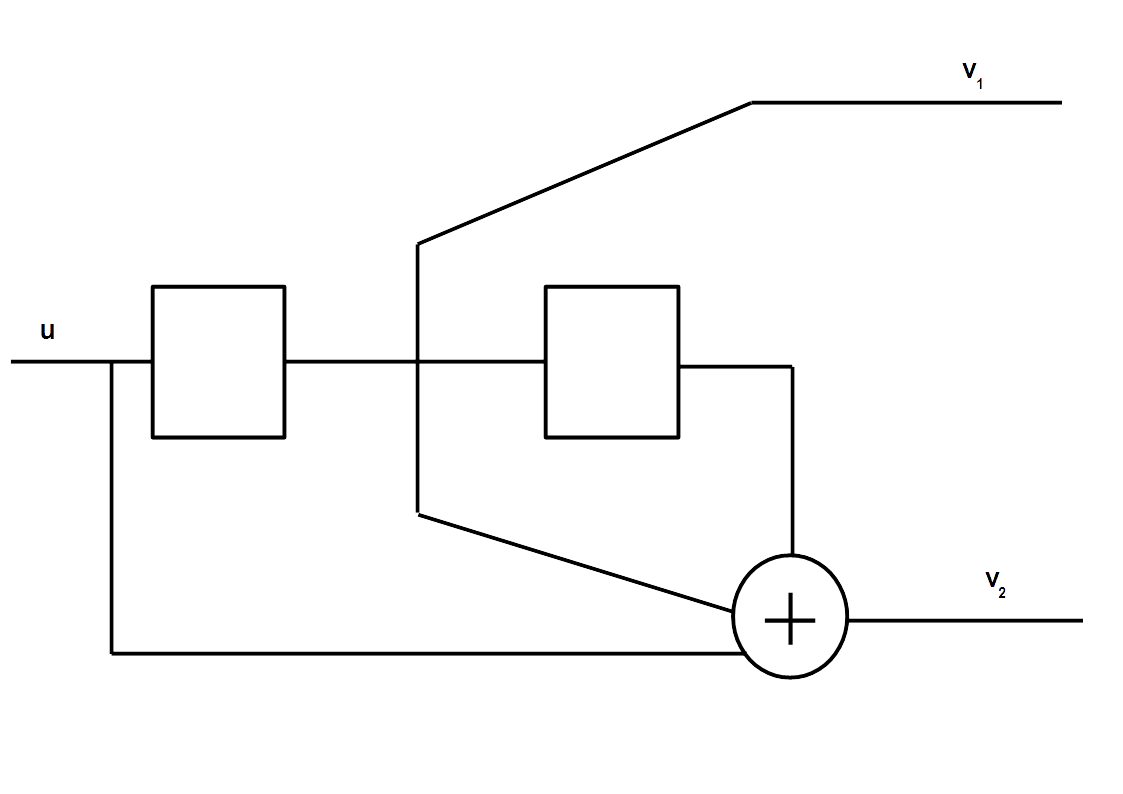
\includegraphics[width=0.4\textwidth]{images/enc}
\caption{Feedforward encoder for the specified convolutional code of memory order 2}
\label{enc}
\end{figure}

\begin{figure}
\centering
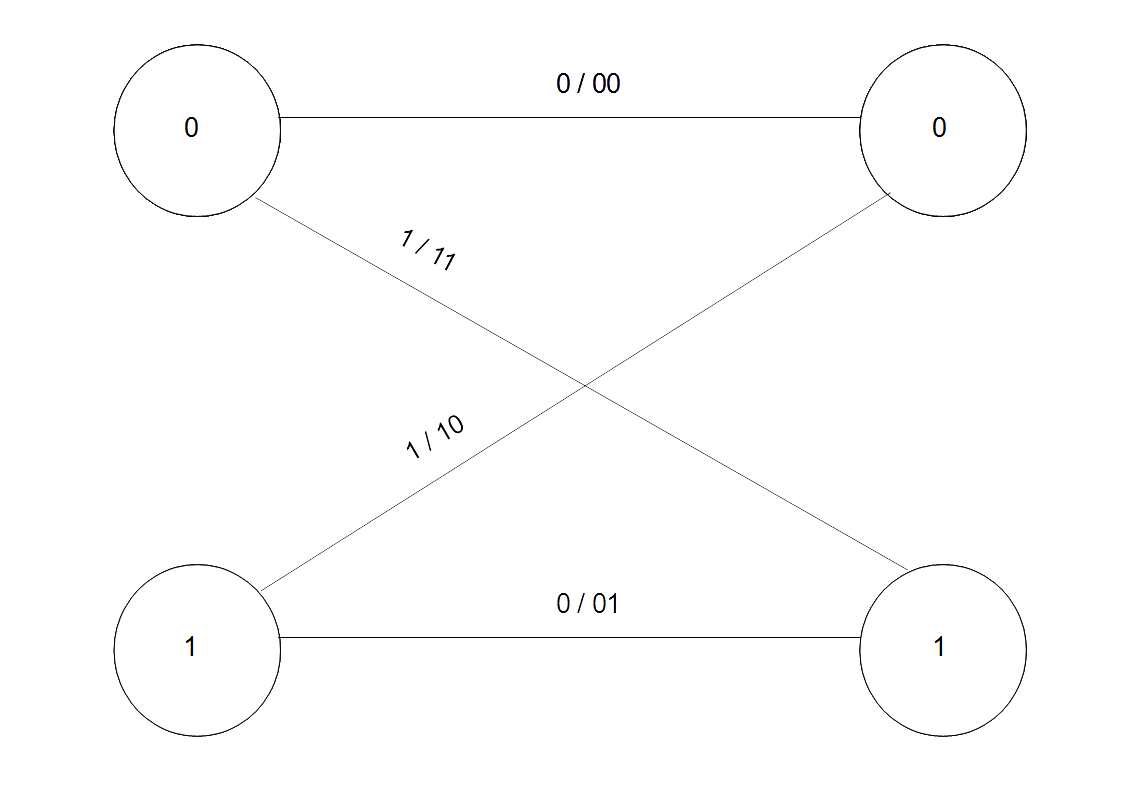
\includegraphics[width=0.4\textwidth]{images/state}
\caption{State Diagram for the convolutional code}
\label{state}
\end{figure}

For the decoding, we assume the all-zero input message. We pass it through the trellis encoder to obtain the output. Note that for an input message of length $10^4$, the codeword length is $N=2(\frac{k}{R}+mem) = 2*10^4 + 4$. 

For code simplicity, we store 2 arrays, one for the state-nextstate-output relations for input 0, and one for input 1. We take the Generator matrix as input, and create the trellis diagram

We then use BPSK modulation to obtain the codeword sent through the channel. We use the code in \cite{AWGN} to simulate the AWGN channel for a given SNR.

\section{Viterbi Decoding} 

We use the soft decision Viterbi-algorithm for decoding. We repeat the state-diagram and trace a path through the trellis corresponding to the shortest distance codeword. Rather than making hard-bit-decisions in each stage, we use a branch-metric, computed by the closeness of the received vector to input $\{0,1\}$. It can be shown that over the AWGN channel, the metric $\frac{2r}{\sigma^2}$ corresponds to the ML decision. So, we just use the metric as $r$, the distance from the outputs corresponding to input $\{0,1\}$, that is we use Euclidian distance as our metric. 
\\ \\
The script used to do this is \textbf{viterbi.m}. We store the path metrics for each state in \textit{SM}. We compute for each state, the branch metrics \textit{BM0,BM1} corresponding to the 2 inputs. We then compute the next state path metric as the smallest metric of incoming branches, stored in \textit{SM\_next}. We check for the path with the smallest metric, and use that to get the closest codeword. 
\pagebreak
It performs encoding decoding, and generates the BER-Curve. We sent a message of length $10^4$. Figure (\ref{ber}) shows the BER-SNR curves. . 

\begin{figure}
\centering
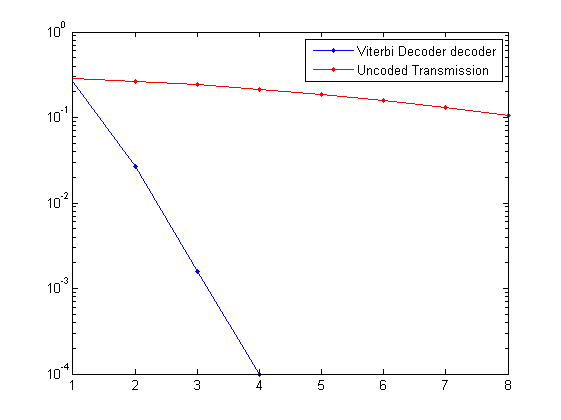
\includegraphics[width=0.8\textwidth]{images/ber3}
\caption{Comparison of BER-SNR curves for the Viterbi Decoder, and Uncoded BPSK transmission}
\label{ber}
\end{figure}

\begin{thebibliography}{155}
\bibitem{AWGN}
AWGN Generation in MATLAB \textit{addAWGN.m} - \\
http://stackoverflow.com/questions/23690766/proper-way-to-add-noise-to-signal
\end{thebibliography}

\end{document}

